\chapter{IMPROVED DUAL-SIM APPROACH TO GATESIM}
\label{chap:dualsim.tex}
Analyzing limitations associated with \emph{early dual-sim approach} shows that the main cause of inefficiency was the method used to capture, store, and applying test vectors onto the netlist. Analyzing limitations associated with \emph{co-sim approach}, it was inferred that the cause was bulky test-bench components associated with RTL simulations. Hence an improved solution would contain minimal testbench components retained and have an efficient method to capture, store, and apply test vectors. 

Test vectors are nothing but signal values at specific point in time. There are already different formats to store this information efficiently. FSDB \nomenclature{FSDB}{Fast Signal Database} is one such format. Hence it was suggested to improve gatesim methodology using FSDB itself as the format to store test vectors. The proposed solution should also improve on

\begin{description}
	\item[Storage requirements] Ensuring that storage resources are effectively used
	\item[Turn-around times] Should avoid re-build for different test vectors
\end{description}

FSDB\cite{SS:Verdi} or Fast Signal Database is a signal data file, similar to VCD\cite{ieee:v:2005} \nomenclature{VCD}{Value Change Dump} but much more compact. This format is in wide use across industry. Quick analysis revealed that FSDB as input test vectors could be accomplished. Existing API's \nomenclature{API}{Application Programming Interface} provided by Verdi\cite{SS:Verdi} tool set for FSDB format could be used to retrieve values from FSDB. PLI$/$VPI\cite{ieee:v:2005} could be used to drive stimulus onto netlist.


The improved methodology becomes a dual-simulation methodology with two separate simulations.
\begin{enumerate}
	\item First simulation with non-gatesim components to generate the test vectors in FSDB format.
	\item Second simulation with only gatesim components with capability to apply test vectors from FSDB directly.
\end{enumerate}



\section {DUAL-SIM FLOW}

\begin{figure}[H]
\centering
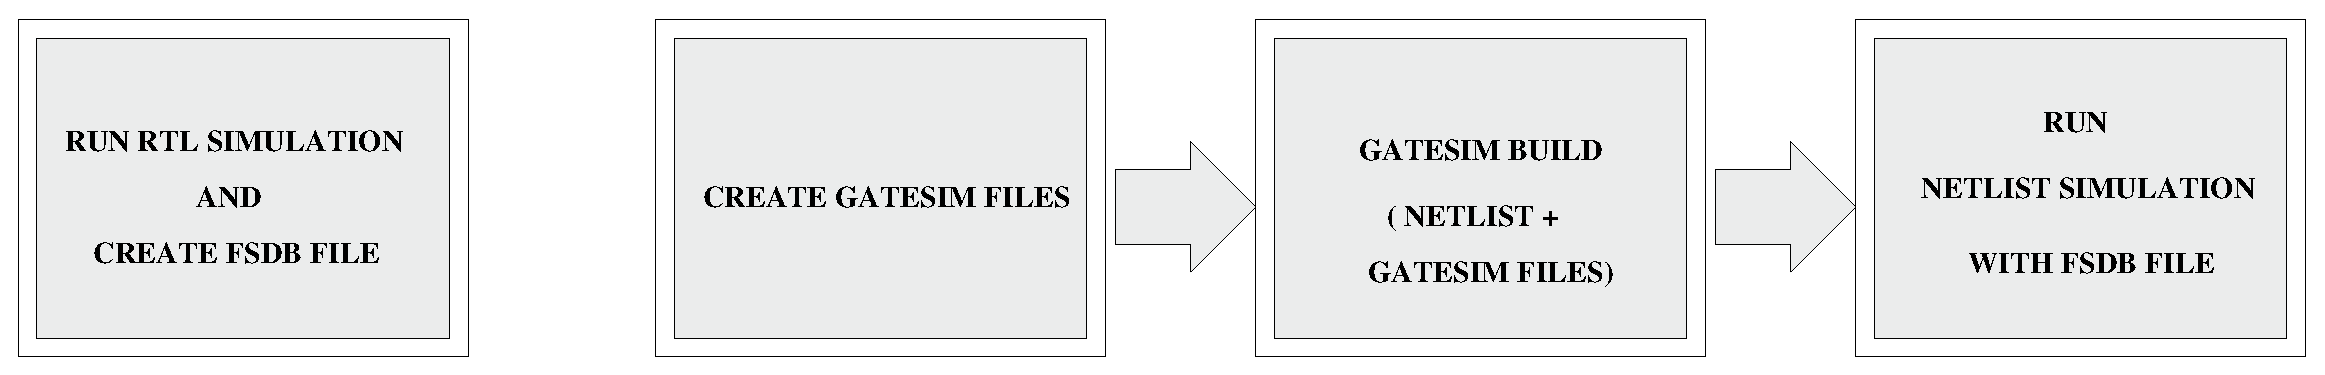
\includegraphics[width=6in, height=1.3in]{./figures/dualsim_flow.eps}
\caption{Dual Sim}
\label{fig:dualsim_flow.eps}
\end{figure}

~\figurename{~\ref{fig:dualsim_flow.eps}} gives the flow of proposed dual-sim approach. Major steps involved in this flow are:

\begin{enumerate}
	\item Run RTL simulation

	RTL simulation is done along with test bench components for generating test vectors and verification. This is the same build for RTL verification stage. The simulation signals needs to be dumped into FSDB and for this the signal dump should be enabled during the run.
	\item As in the case of co simulation, Gatesim files need to be generated from input files obtained from LEC. Same infrastructure used in co-sim can be used for this.
	\item Get the gatesim build. Here the build structure will have the netlist and gatesim files only. RTL and the bulky testbench components are absent.
	\item Run simulation with specific FSDB file.
\end{enumerate}


\section{IMPLEMENTATION}

Implementation of dual-sim flow involves two major stages: accessing test vectors from FSDB and driving the test vectors onto the netlist input for netlist simulation.
\subsection{USING FSDB AS TEST VECTORS}
\begin{figure}[H]
\centering
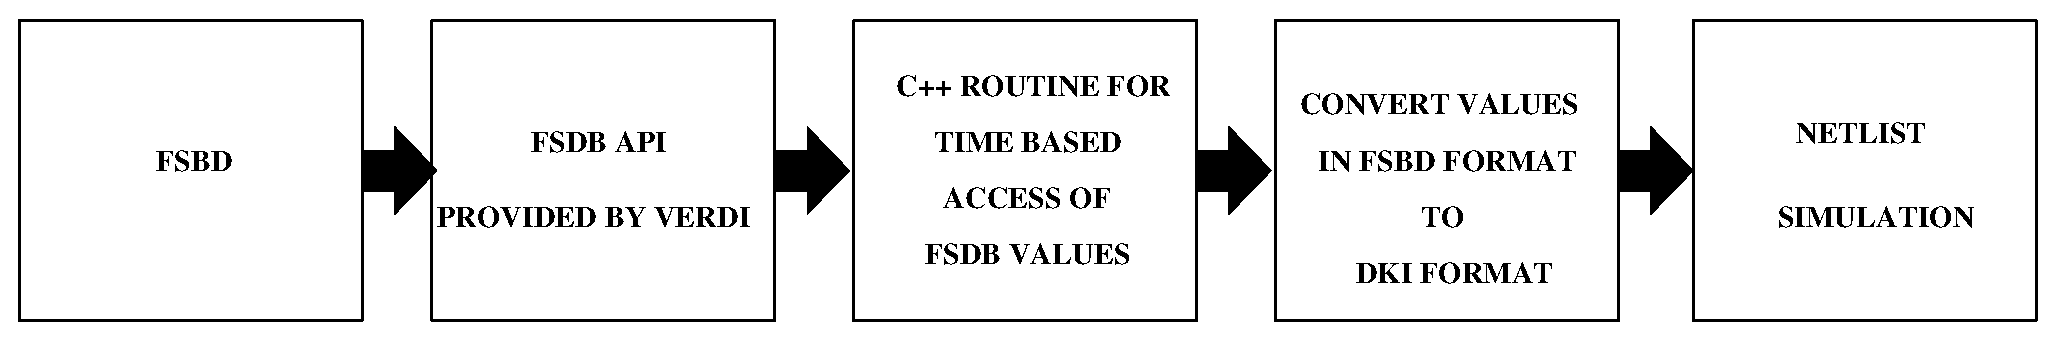
\includegraphics[width=5in, height=1.3in]{./figures/fsdb.eps}
\caption{Accessing FSDB Signals}
\label{fig:fsdb.eps}
\end{figure}

~\figurename{~\ref{fig:fsdb.eps}} shows how test vectors are obtained from .fsdb file and attached onto the netlist simulation flow. The various stages involved are explained below.
\paragraph{Extracting data from FSDB:}FSDB API's are available, which enable signal access. However a larger C++ infrastructure is required for accessing signals for gatesim because of the following reasons:
\begin{enumerate}
	\item Values contained in FSDB needs to be accessed in time-based fashion.
	\item Typical netlist contained hundreds of stimulus points with many wider bus-signals.
\end{enumerate}

\paragraph{Convert FSDB format to DKI format}:C++ infrastructure also needs to convert FSDB format to DKI format. 
Direct Kernel Interface aka DKI is a feature to make available internal kernel data structures. DKI will access intenal variable values andVPI objects are created for simulator-C++ interaction.

VPI or Verilog Procedural Interface is a Verilog- C interface. It was initially known as PLI 2.0.It allows behavioral Verilog code to invoke C functions, and C functions to invoke standard Verilog system tasks. [Wikipedia] In order to drive the verilog netlist the FSDB format need to be converted to VPI format

\paragraph{Drive the netlist}:Drive the netlist using VPI objects that attach C++ signals to verilog signals. 

\subsection{NETLIST SIMULATION FLOW}
\begin{figure}[H]
\centering
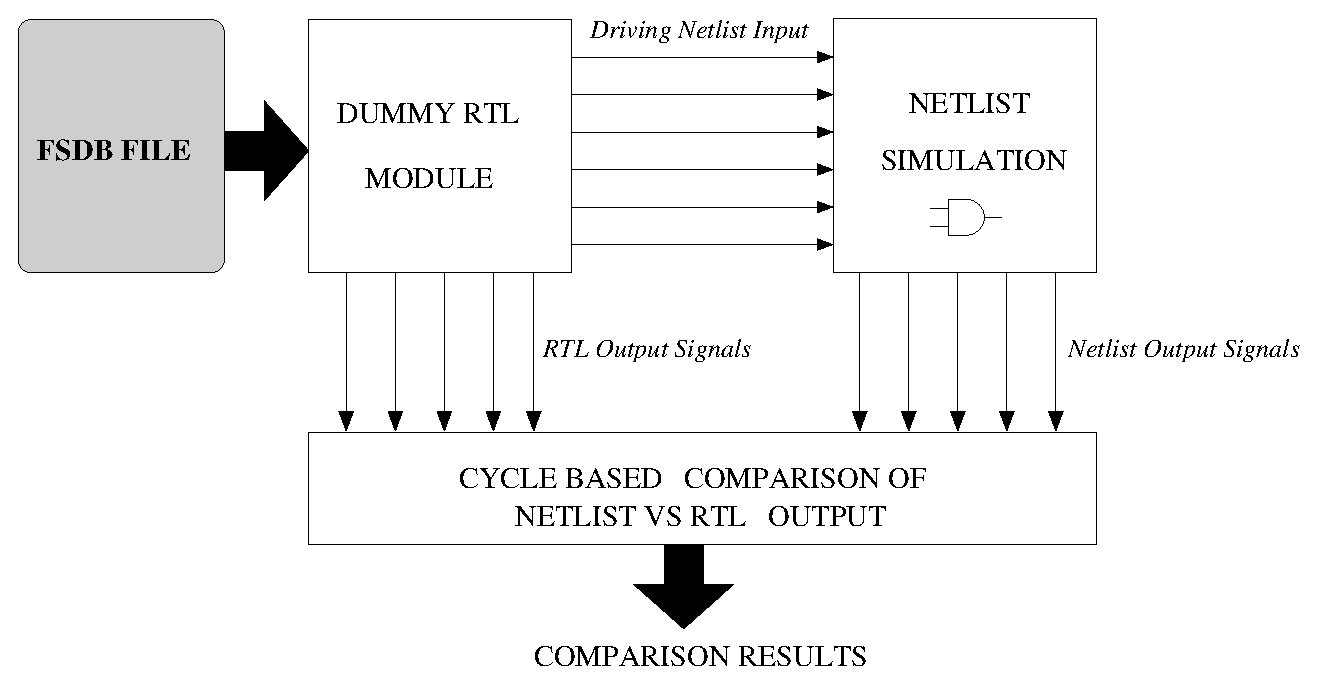
\includegraphics[width=5in, height=3.5in]{./figures/dualsim_sim.eps}
\caption{Netlist Simulation}
\label{fig:dualsim_sim.eps}
\end{figure}

~\figurename{~\ref{fig:dualsim_sim.eps}} show how test vectors are applied onto the netlist and how final comparison is done. Features of Improved gatesim methodology are:
\begin{enumerate}
	\item Obtain test vectors from FSDB; access it in time-based fashion.
	\item Drive stimulus onto a dummy RTL. This dummy RTL does not have any logic other than Input/output. All the input and output ports of the module netlist are included in this dummy RTL module. 
	\item Dummy RTL drives netlist stimulus and other stimulus points inside design (like fuses, un init flops).
	\item Apply appropriate force signals from FSDB directly on to the dummy RTL. The dummy RTL signal forces the netlist signals.
	\item Accomplish verification goals by cycle-comparing netlist behavior to that of its counterpart RTL (as available in the FSDB).
\end{enumerate}
It should be noted that the improved methodology is still dependent on vectors from RTL simulations and is not independent by itself. But gains obtained in turn-around times were of great benefit.



